\documentclass[border=4pt]{standalone}
\usepackage{tikz}
\usepackage{amsmath,amssymb}
\usepackage{mathptmx}
\usetikzlibrary{arrows.meta,positioning,calc,shapes.geometric,decorations.pathreplacing,shadows,fadings,patterns}
\definecolor{cblue}{HTML}{1F4E9C}
\definecolor{cgold}{HTML}{D08C00}
\definecolor{cred}{HTML}{B5172E}
\definecolor{cgreen}{HTML}{1B7A3A}
\definecolor{cgrey}{HTML}{555555}
\definecolor{cpurple}{HTML}{5B2A86}
% oblique 3D cuboid: \cuboid{x}{y}{z}{dx}{dy}{dz}{colour}
\newcommand{\cuboid}[7]{%
  \fill[#7!55!white,draw=#7!60!black,line width=0.4pt] (#1,#2,#3+#6) -- ++(#4,0,0) -- ++(0,#5,0) -- ++(-#4,0,0) -- cycle;
  \fill[#7!80!black,draw=#7!60!black,line width=0.4pt] (#1+#4,#2,#3) -- ++(0,#5,0) -- ++(0,0,#6) -- ++(0,-#5,0) -- cycle;
  \fill[#7,draw=#7!60!black,line width=0.4pt] (#1,#2,#3) -- ++(#4,0,0) -- ++(0,0,#6) -- ++(-#4,0,0) -- cycle;}

\begin{document}
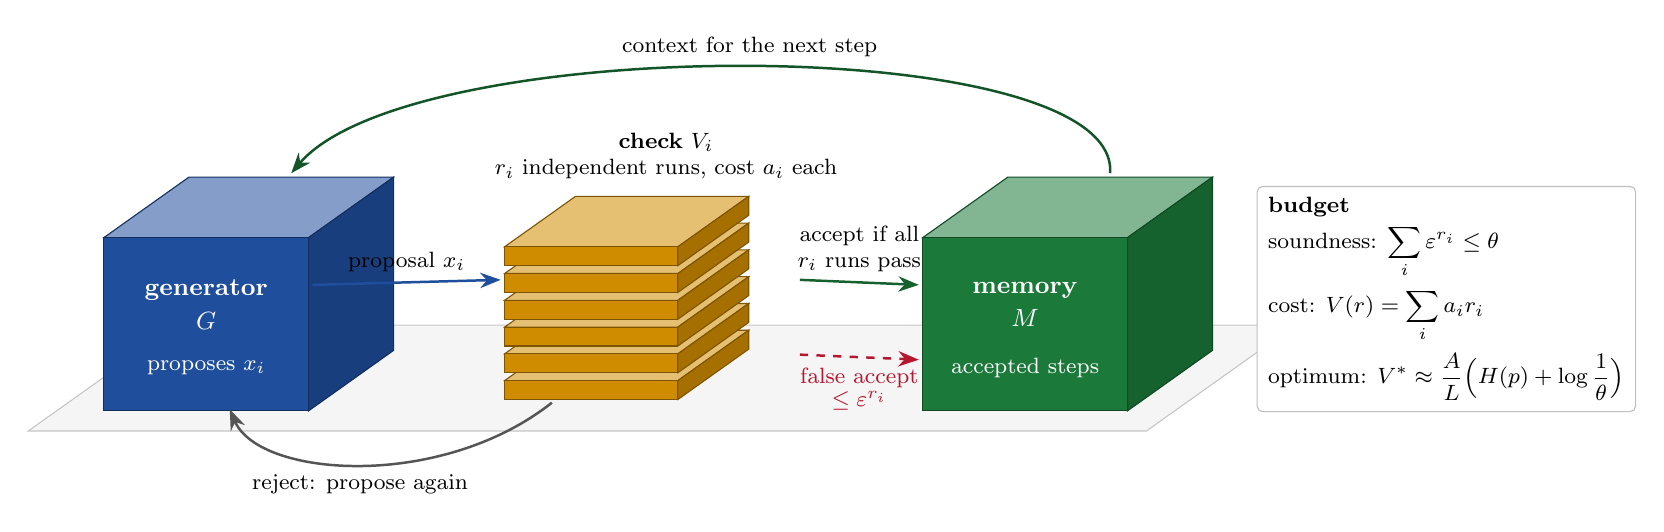
\begin{tikzpicture}[x={(1cm,0cm)},y={(0.45cm,0.32cm)},z={(0cm,1cm)},
  lab/.style={font=\small,align=center},
  arr/.style={-{Stealth[length=2.6mm]},line width=0.9pt}]
% ground plate
\fill[gray!8,draw=gray!45] (-0.6,-0.8,0) -- (13.6,-0.8,0) -- (13.6,3.4,0) -- (-0.6,3.4,0) -- cycle;
% generator
\cuboid{0}{0}{0}{2.6}{2.4}{2.2}{cblue}
\node[lab,white] at (1.3,0,1.35) {\textbf{generator}\\[1pt] $G$};
\node[lab,white,font=\footnotesize] at (1.3,0,0.55) {proposes $x_i$};
% checks: stacked plates for r_i repetitions
\foreach \j in {0,...,5}{
  \pgfmathsetmacro\zz{0.08+0.34*\j}
  \cuboid{5.0}{0.2}{\zz}{2.2}{2.0}{0.24}{cgold}}
\node[lab,font=\footnotesize] at (6.6,1.2,2.85) {\textbf{check} $V_i$\\ $r_i$ independent runs, cost $a_i$ each};
% memory
\cuboid{10.4}{0}{0}{2.6}{2.4}{2.2}{cgreen}
\node[lab,white] at (11.7,0,1.35) {\textbf{memory}\\[1pt] $M$};
\node[lab,white,font=\footnotesize] at (11.7,0,0.55) {accepted steps};
% arrows
\draw[arr,cblue] (2.65,0,1.6) -- node[above,font=\footnotesize,black] {proposal $x_i$} (4.95,0.2,1.6);
\draw[arr,cgreen!80!black] (8.75,0.2,1.6) -- node[above,font=\footnotesize,black,align=center] {accept if all\\ $r_i$ runs pass} (10.35,0,1.6);
\draw[arr,cred,dashed] (8.75,0.2,0.65) -- node[below,font=\footnotesize,cred,align=center] {false accept\\[-1pt] $\le\varepsilon^{r_i}$} (10.35,0,0.65);
\draw[arr,cgrey] (5.6,0.2,0.04) .. controls (5.0,-1.6,-0.5) and (2.6,-1.4,-0.4) .. node[below,font=\footnotesize,black,pos=0.5] {reject: propose again} (1.6,0,0.02);
\draw[arr,cgreen!70!black] (11.7,2.4,2.25) .. controls (11.2,3.8,3.6) and (2.2,3.8,3.6) .. node[above,font=\footnotesize,black] {context for the next step} (1.3,2.4,2.25);
% cost ledger on the right
\node[font=\footnotesize,align=left,draw=gray!50,fill=white,rounded corners=2pt,inner sep=4pt] at (16.6,1.0,1.1)
 {\textbf{budget}\\[2pt]
  soundness: $\displaystyle\sum_i\varepsilon^{r_i}\le\theta$\\[3pt]
  cost: $\displaystyle V(r)=\sum_i a_i r_i$\\[3pt]
  optimum: $\displaystyle V^*\approx\frac{A}{L}\Bigl(H(p)+\log\frac1\theta\Bigr)$};
\end{tikzpicture}
\end{document}
